% Options for packages loaded elsewhere
% Options for packages loaded elsewhere
\PassOptionsToPackage{unicode}{hyperref}
\PassOptionsToPackage{hyphens}{url}
\PassOptionsToPackage{dvipsnames,svgnames,x11names}{xcolor}
%
\documentclass[
  british,
  a4paper,
]{article}
\usepackage{xcolor}
\usepackage{amsmath,amssymb}
\setcounter{secnumdepth}{-\maxdimen} % remove section numbering
\usepackage{iftex}
\ifPDFTeX
  \usepackage[T1]{fontenc}
  \usepackage[utf8]{inputenc}
  \usepackage{textcomp} % provide euro and other symbols
\else % if luatex or xetex
  \usepackage{unicode-math} % this also loads fontspec
  \defaultfontfeatures{Scale=MatchLowercase}
  \defaultfontfeatures[\rmfamily]{Ligatures=TeX,Scale=1}
\fi
\usepackage{lmodern}
\ifPDFTeX\else
  % xetex/luatex font selection
\fi
% Use upquote if available, for straight quotes in verbatim environments
\IfFileExists{upquote.sty}{\usepackage{upquote}}{}
\IfFileExists{microtype.sty}{% use microtype if available
  \usepackage[]{microtype}
  \UseMicrotypeSet[protrusion]{basicmath} % disable protrusion for tt fonts
}{}
\makeatletter
\@ifundefined{KOMAClassName}{% if non-KOMA class
  \IfFileExists{parskip.sty}{%
    \usepackage{parskip}
  }{% else
    \setlength{\parindent}{0pt}
    \setlength{\parskip}{6pt plus 2pt minus 1pt}}
}{% if KOMA class
  \KOMAoptions{parskip=half}}
\makeatother
% Make \paragraph and \subparagraph free-standing
\makeatletter
\ifx\paragraph\undefined\else
  \let\oldparagraph\paragraph
  \renewcommand{\paragraph}{
    \@ifstar
      \xxxParagraphStar
      \xxxParagraphNoStar
  }
  \newcommand{\xxxParagraphStar}[1]{\oldparagraph*{#1}\mbox{}}
  \newcommand{\xxxParagraphNoStar}[1]{\oldparagraph{#1}\mbox{}}
\fi
\ifx\subparagraph\undefined\else
  \let\oldsubparagraph\subparagraph
  \renewcommand{\subparagraph}{
    \@ifstar
      \xxxSubParagraphStar
      \xxxSubParagraphNoStar
  }
  \newcommand{\xxxSubParagraphStar}[1]{\oldsubparagraph*{#1}\mbox{}}
  \newcommand{\xxxSubParagraphNoStar}[1]{\oldsubparagraph{#1}\mbox{}}
\fi
\makeatother


\usepackage{longtable,booktabs,array}
\newcounter{none} % for unnumbered tables
\usepackage{calc} % for calculating minipage widths
% Correct order of tables after \paragraph or \subparagraph
\usepackage{etoolbox}
\makeatletter
\patchcmd\longtable{\par}{\if@noskipsec\mbox{}\fi\par}{}{}
\makeatother
% Allow footnotes in longtable head/foot
\IfFileExists{footnotehyper.sty}{\usepackage{footnotehyper}}{\usepackage{footnote}}
\makesavenoteenv{longtable}
\usepackage{graphicx}
\makeatletter
\newsavebox\pandoc@box
\newcommand*\pandocbounded[1]{% scales image to fit in text height/width
  \sbox\pandoc@box{#1}%
  \Gscale@div\@tempa{\textheight}{\dimexpr\ht\pandoc@box+\dp\pandoc@box\relax}%
  \Gscale@div\@tempb{\linewidth}{\wd\pandoc@box}%
  \ifdim\@tempb\p@<\@tempa\p@\let\@tempa\@tempb\fi% select the smaller of both
  \ifdim\@tempa\p@<\p@\scalebox{\@tempa}{\usebox\pandoc@box}%
  \else\usebox{\pandoc@box}%
  \fi%
}
% Set default figure placement to htbp
\def\fps@figure{htbp}
\makeatother



\ifLuaTeX
\usepackage[bidi=basic,shorthands=off]{babel}
\else
\usepackage[bidi=default,shorthands=off]{babel}
\fi
\ifLuaTeX
  \usepackage{selnolig} % disable illegal ligatures
\fi


\setlength{\emergencystretch}{3em} % prevent overfull lines

\providecommand{\tightlist}{%
  \setlength{\itemsep}{0pt}\setlength{\parskip}{0pt}}



 


\makeatletter
\@ifpackageloaded{tcolorbox}{}{\usepackage[skins,breakable]{tcolorbox}}
\@ifpackageloaded{fontawesome5}{}{\usepackage{fontawesome5}}
\definecolor{quarto-callout-color}{HTML}{909090}
\definecolor{quarto-callout-note-color}{HTML}{0758E5}
\definecolor{quarto-callout-important-color}{HTML}{CC1914}
\definecolor{quarto-callout-warning-color}{HTML}{EB9113}
\definecolor{quarto-callout-tip-color}{HTML}{00A047}
\definecolor{quarto-callout-caution-color}{HTML}{FC5300}
\definecolor{quarto-callout-color-frame}{HTML}{acacac}
\definecolor{quarto-callout-note-color-frame}{HTML}{4582ec}
\definecolor{quarto-callout-important-color-frame}{HTML}{d9534f}
\definecolor{quarto-callout-warning-color-frame}{HTML}{f0ad4e}
\definecolor{quarto-callout-tip-color-frame}{HTML}{02b875}
\definecolor{quarto-callout-caution-color-frame}{HTML}{fd7e14}
\makeatother
\makeatletter
\@ifpackageloaded{caption}{}{\usepackage{caption}}
\AtBeginDocument{%
\ifdefined\contentsname
  \renewcommand*\contentsname{Table of contents}
\else
  \newcommand\contentsname{Table of contents}
\fi
\ifdefined\listfigurename
  \renewcommand*\listfigurename{List of Figures}
\else
  \newcommand\listfigurename{List of Figures}
\fi
\ifdefined\listtablename
  \renewcommand*\listtablename{List of Tables}
\else
  \newcommand\listtablename{List of Tables}
\fi
\ifdefined\figurename
  \renewcommand*\figurename{Figure}
\else
  \newcommand\figurename{Figure}
\fi
\ifdefined\tablename
  \renewcommand*\tablename{Table}
\else
  \newcommand\tablename{Table}
\fi
}
\@ifpackageloaded{float}{}{\usepackage{float}}
\floatstyle{ruled}
\@ifundefined{c@chapter}{\newfloat{codelisting}{h}{lop}}{\newfloat{codelisting}{h}{lop}[chapter]}
\floatname{codelisting}{Listing}
\newcommand*\listoflistings{\listof{codelisting}{List of Listings}}
\makeatother
\makeatletter
\makeatother
\makeatletter
\@ifpackageloaded{caption}{}{\usepackage{caption}}
\@ifpackageloaded{subcaption}{}{\usepackage{subcaption}}
\makeatother
\usepackage{bookmark}
\IfFileExists{xurl.sty}{\usepackage{xurl}}{} % add URL line breaks if available
\urlstyle{same}
% fallback for those not using the hyperref driver hyperxmp:
\makeatletter
\@ifundefined{xmpquote}{\newcommand{\xmpquote}[1]{#1}}{}
\makeatother
\hypersetup{
  pdftitle={Central Europe's industrial drift from Germany},
  pdfauthor={Carlos Galindo},
  pdflang={en-GB},
  colorlinks=true,
  linkcolor={blue},
  filecolor={Maroon},
  citecolor={Blue},
  urlcolor={Blue},
  pdfcreator={LaTeX via pandoc}}


\title{Central Europe's industrial drift from Germany}
\usepackage{etoolbox}
\makeatletter
\providecommand{\subtitle}[1]{% add subtitle to \maketitle
  \apptocmd{\@title}{\par {\large #1 \par}}{}{}
}
\makeatother
\subtitle{A gradual decoupling, not a structural break, and a policy
rate close to its rule}
\author{Carlos Galindo}
\date{}
\begin{document}
\maketitle


\begin{tcolorbox}[enhanced jigsaw, arc=.35mm, bottomrule=.15mm, breakable, colback=white, colframe=quarto-callout-note-color-frame, left=2mm, leftrule=.75mm, opacityback=0, rightrule=.15mm, toprule=.15mm]

\vspace{-3mm}\textbf{At a glance}\vspace{3mm}

\begin{itemize}
\tightlist
\item
  \textbf{Question.} Since 2022, have industrial economies in Poland,
  Hungary and Czechia broken away from Germany, and which of the
  competing stories about Polish industry, public finances and interest
  rates survives contact with the data?
\item
  \textbf{Approach.} Monthly industrial output compared with Germany in
  growth terms, rolling correlations, formal break tests at
  pre-specified dates, a margin proxy from producer prices and labour
  costs, and a Taylor-rule check of the Polish policy rate.
\item
  \textbf{Finding.} The drift is real and large in levels, but the break
  tests find no discrete break. The pattern is a gradual decoupling, and
  the evidence supports volume strength and margin weakness at the same
  time.
\item
  \textbf{Why it matters.} ``Structural decay'' and ``cyclical rebound''
  are often argued as rivals. Here they describe different dimensions of
  one economy.
\end{itemize}

\end{tcolorbox}

\subsection{The question}\label{the-question}

Central European manufacturing has long been wired into German supply
chains, so for two decades the three economies were treated as an
extension of the German cycle. Since 2022 that assumption has been under
pressure. Germany absorbed an energy-price shock that hit its industrial
base hard, while Poland in particular kept growing. Commentary quickly
split into camps: one says Polish industry is in structural decay,
another says it is a cyclical rebound; one says Polish public finances
are an institutional strength, another says they are a sovereign-risk
problem; one says the central bank is prudent, another says it is
procrastinating.

The obvious way to settle such arguments is to pick the indicator that
supports your side. This project does the opposite. It states each
narrative as a testable null, chooses the evidence that could embarrass
it, and reports where the data are silent. The audience is anyone who
has to form a view on the region quickly, whether an economist, an
investor or a policy reader, and needs to know which claims are safe to
repeat.

\subsection{Approach}\label{approach}

\textbf{Data.} Monthly industrial output, producer prices, retail trade
and consumer prices for Poland, Hungary, Czechia and Germany, with
quarterly labour-cost indices, policy rates and long-term government
bond yields, all from official statistical sources. The monthly panel
covers 62 series. Growth is always measured as
three-month-on-three-month change on seasonally adjusted data, never as
year-on-year change, which blurs turning points.

\textbf{Divergence.} Each country's industrial output was indexed to its
December 2019 level and compared with Germany. The co-movement of Polish
and German output growth was tracked with a rolling 24-month
correlation, split into a pre-pandemic, a pandemic-synchronisation and a
post-2022 window. A single-factor decomposition of the four output
series gave the share of common variation.

\textbf{Narrative tests.} For the industry narrative, the null was that
the divergence is cyclical and will revert as energy prices normalise.
It was tested with Chow tests for a shift in the growth relationship at
three pre-specified dates: the financial crisis, the pandemic and the
2022 energy shock. For competitiveness, a margin proxy was built as the
gap between output-price and wage-cost indices. For public finances,
bond spreads and real yields were examined. For monetary policy, the
policy rate was compared with a Taylor rule using inflation, an output
measure and unemployment, with an assumed neutral real rate of 3.5 per
cent.

\textbf{Checks.} Every result was reported with its sample length and
its power limits, and each claim was classed as structural or cyclical
only against an explicit multi-cycle standard. Where a figure came from
outside the dataset, it was labelled as context and not used in a test.

\subsection{What the work shows}\label{what-the-work-shows}

\subsubsection{The levels have moved
apart}\label{the-levels-have-moved-apart}

Measured against December 2019, Polish industrial output stands 18.2 per
cent higher, Hungarian 3.1 per cent higher and Czech 1.2 per cent
higher, while German output is 6.7 per cent lower. That is a large
reallocation of European manufacturing in four years, and it is the fact
that fuels the structural-decay and structural-shift stories alike.

\begin{figure}

\centering{

\pandocbounded{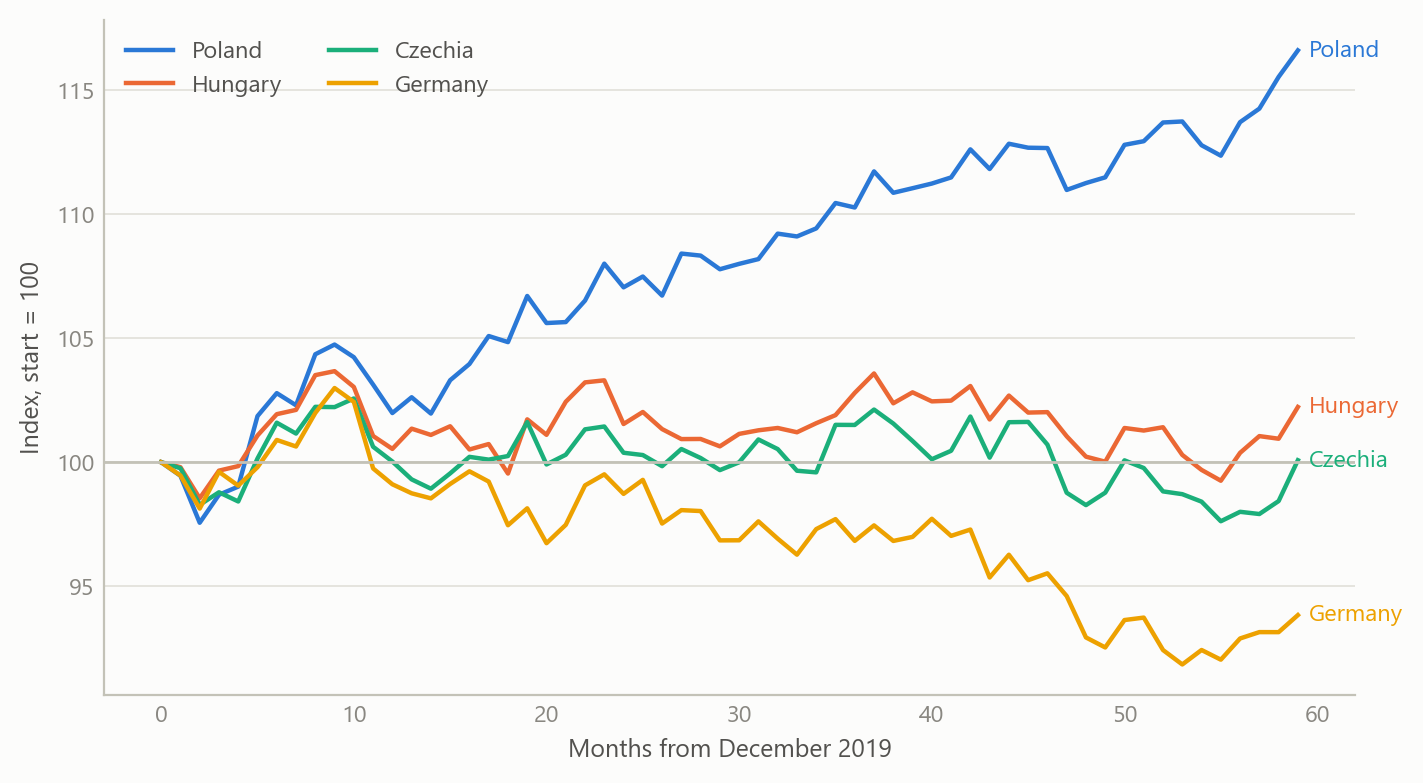
\includegraphics[keepaspectratio]{index_files/figure-latex/fig-levels-output-1.png}}

}

\caption{\label{fig-levels}Industrial output indexed to December 2019 =
100, four economies, monthly (simulated data).}

\end{figure}%

\subsubsection{Co-movement fell, but not to a
break}\label{co-movement-fell-but-not-to-a-break}

The correlation of Polish and German output growth is the sharpest
single piece of evidence. It was strongly positive in the pandemic
window, at about +0.92, when synchronised closures and reopenings moved
everything together. In the post-2022 window its average was +0.39, and
the latest reading was -0.67. A first reading of the last value says the
link has inverted. A fuller reading says the window average is still
positive, and the latest value may be the tail of the energy shock and
not a permanent state. The single-factor share is also misleading: it is
dominated by the pandemic crash and rebound, so a high full-sample
common share coexists with a weaker post-2022 link.

\begin{figure}

\centering{

\pandocbounded{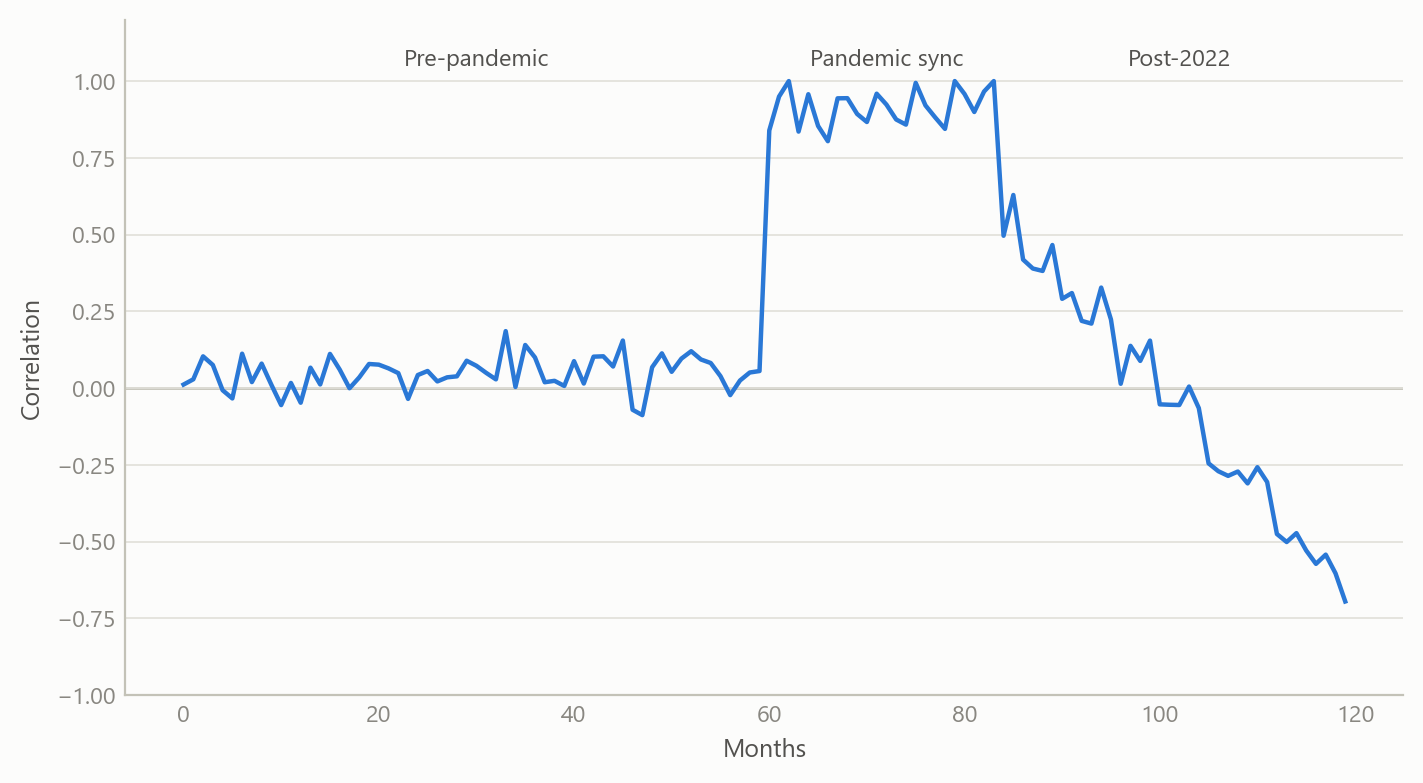
\includegraphics[keepaspectratio]{index_files/figure-latex/fig-corr-output-1.png}}

}

\caption{\label{fig-corr}Rolling 24-month correlation of Polish and
German output growth, three regimes (simulated data).}

\end{figure}%

\subsubsection{No discrete break}\label{no-discrete-break}

Output growth momentum slowed from a pre-2022 mean of +0.448 per cent to
a post-2022 mean of +0.147 per cent per quarter-on-quarter-style step, a
shift of about 0.30 percentage points, which is meaningful but not
catastrophic. The Chow tests at the three pre-specified dates give
p-values of 0.22 for the financial crisis, 0.69 for the pandemic and
0.23 for the 2022 shock. None is significant. The slowdown is gradual.
That is the basis for the headline: a gradual decoupling, not a
structural break. The tests are honest about their limits: the
post-shock sample is only a few dozen months, so low power could hide a
real change, and the null of a cyclical divergence cannot be rejected
either.

\subsubsection{Volume strength, margin
weakness}\label{volume-strength-margin-weakness}

The margin proxy, output prices less wage costs, is where the picture
turns. Germany is the only economy in which output prices exceed wage
costs, by 15.5 points. Poland's gap is -45.4 points, Hungary's -23.9 and
Czechia's -10.3. Poland therefore shows the strongest volume growth and
the weakest margin at once. This resolves much of the ``structural decay
versus cyclical rebound'' argument: decay refers to margins and
competitiveness, rebound to output volume, and both can be true when
growth is driven by wages and not by pricing power. The proxy is not a
firm-level margin, so it is a direction-of-pressure indicator and
nothing more.

\begin{figure}

\centering{

\pandocbounded{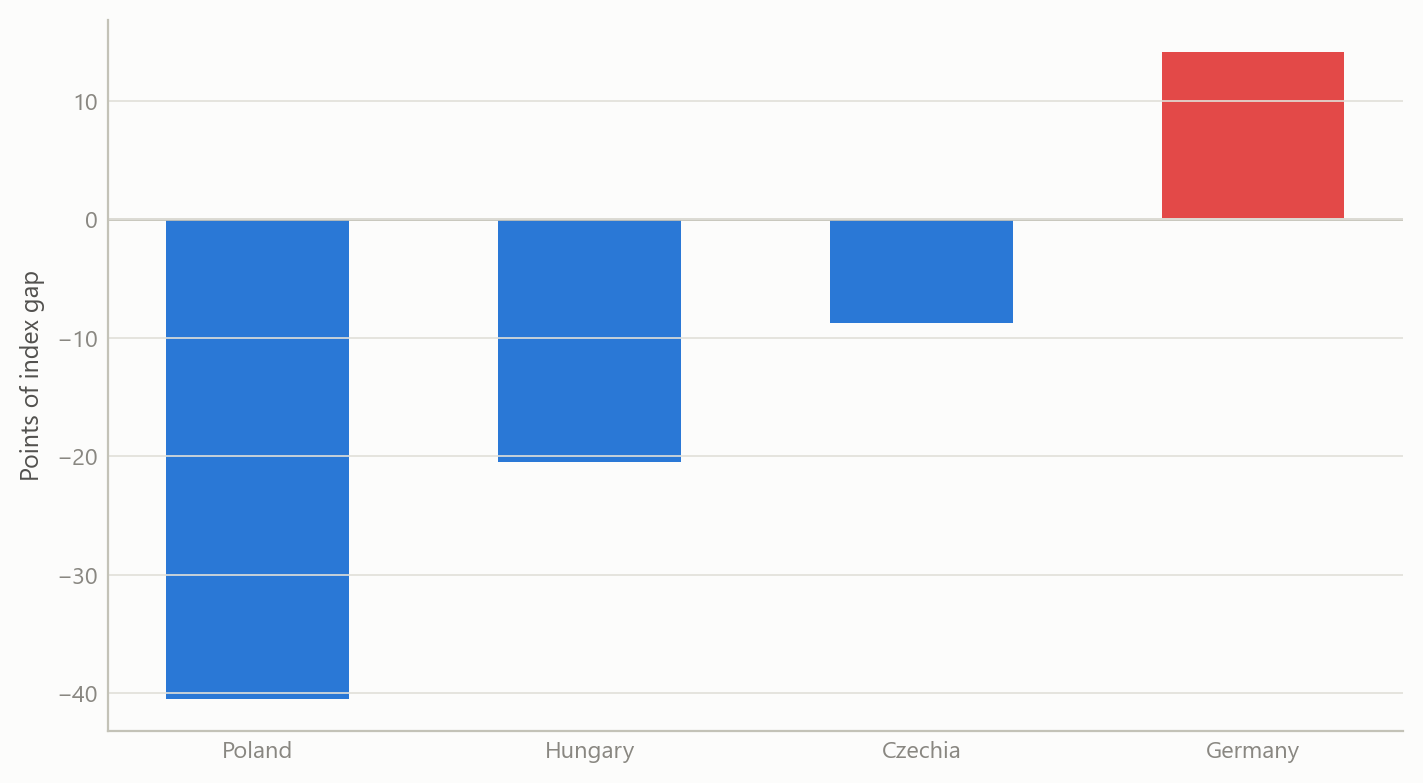
\includegraphics[keepaspectratio]{index_files/figure-latex/fig-margin-output-1.png}}

}

\caption{\label{fig-margin}Margin proxy, output-price index minus
wage-cost index, four economies (simulated data).}

\end{figure}%

\subsubsection{A policy rate close to its
rule}\label{a-policy-rate-close-to-its-rule}

For the Polish policy rate, the last full-data observation, December
2023, was 5.54 per cent against a Taylor-rule value of 5.41 per cent
with the assumed neutral rate. The gap of 0.13 points means policy was
essentially neutral by that standard. In the later data vintage the
central bank cut by 175 basis points between May and December 2025 while
its Hungarian peer held its rate throughout and the Czech bank cut a
quarter point. Three different strategies followed similar inflation
convergence. The rule explains little on its own: in the broader panel
regression, output variation is almost entirely idiosyncratic, with an
R-squared of about 0.03 on 853 observations. And the conclusion is
conditional on the neutral rate, which was assumed, not estimated.

\begin{figure}

\centering{

\pandocbounded{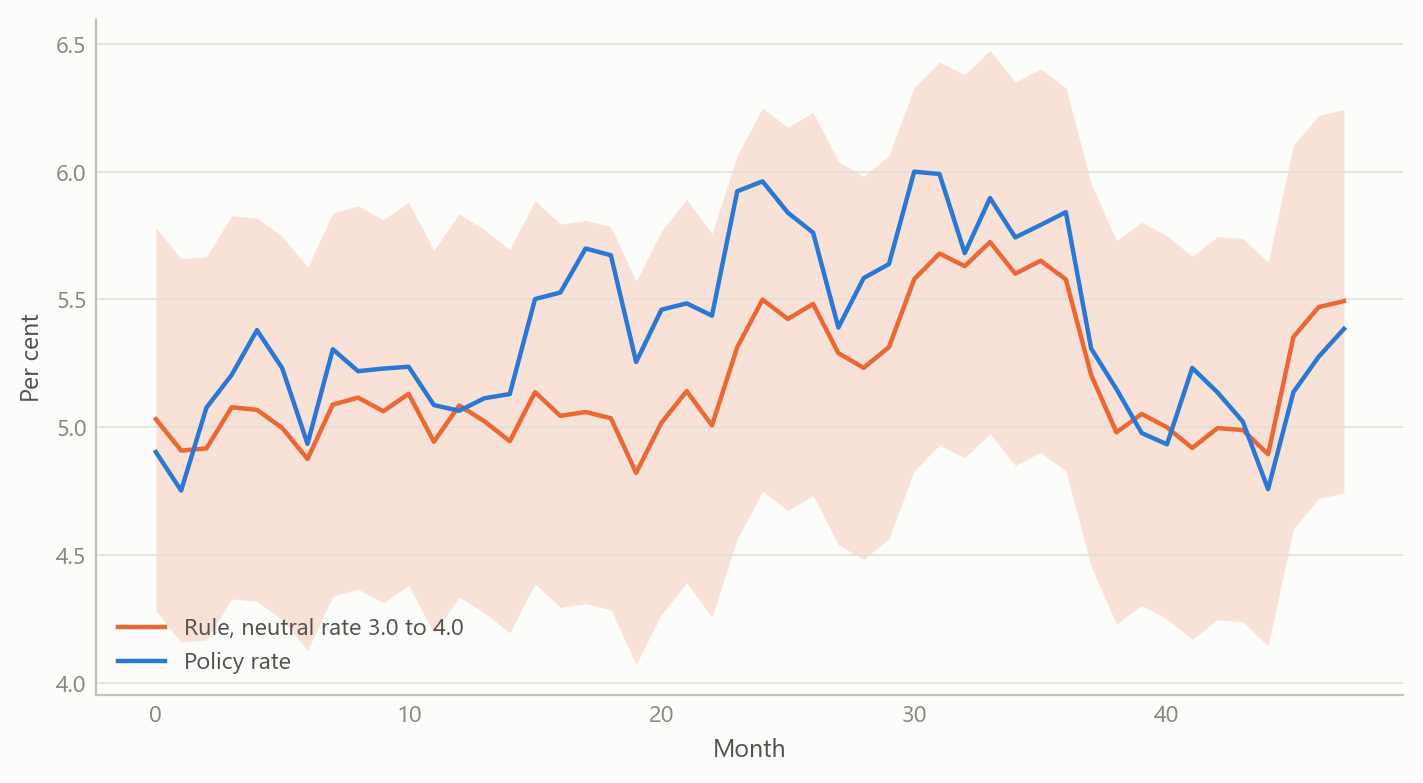
\includegraphics[keepaspectratio]{index_files/figure-latex/fig-taylor-output-1.png}}

}

\caption{\label{fig-taylor}Policy rate against a Taylor-rule band for a
range of neutral rates (simulated data).}

\end{figure}%

\subsection{Insights}\label{insights}

\begin{enumerate}
\def\labelenumi{\arabic{enumi}.}
\tightlist
\item
  \textbf{Level divergence and dynamic decoupling are different claims.}
  Output levels diverge sharply, while growth co-movement fades
  gradually. Arguing from the first to a ``structural'' label skips a
  step.
\item
  \textbf{Volume and margins can point in opposite directions.} The most
  polarising economy in the group is polarising because its volume and
  margin indicators disagree, so analysts disagree for good reason.
\item
  \textbf{A last observation is not a regime.} The latest correlation
  value is far below the window average. Reporting both keeps a tail
  event from being read as a permanent state.
\item
  \textbf{A rule check is only as good as its neutral rate.} Fixing the
  neutral rate makes the verdict a conditional statement. The honest
  output is a band, not a point.
\item
  \textbf{Say what cannot be tested.} Public finances could be discussed
  only through bond pricing, because no fiscal balance or debt series
  was in the dataset. The fiscal narrative was therefore left as
  plausible on both sides, with bond yields placing Poland between
  Czechia and Hungary.
\end{enumerate}

\subsection{Limits and next steps}\label{limits-and-next-steps}

The post-2022 sample is short, so break tests have low power. A calendar
of two full business cycles would be needed to call any change
structural, and that is not available. Output and policy-rate series
ended earlier than prices and labour costs in the vintage used, so some
results are as of an earlier date and a few current-state figures came
from outside the dataset and were used as context only. The margin proxy
is an index gap, not firm-level profit. Real rates use realised
inflation, not expectations, and yield spreads mix sovereign risk with
monetary stance. The next step is a refresh to a common end date, a
sensitivity band on the neutral rate, and a longer window.

\subsection{About the evidence}\label{about-the-evidence}

The analysis is a 2026 piece of independent work built on official
monthly and quarterly statistics for four economies, with 62 series and
837 months at the longest. The figures in this note are illustrative
simulations that share the structure of the real analysis. The numbers
in the text are the project's own results.

Figures and tables marked \emph{simulated} are generated from simulated
data built to share the structure of the analysis (its variables,
horizons and frequencies). They show how the method works and what its
output looks like; they are not the project's results. Results stated in
the text are the project's own. Methods are described at the level of a
methods section. Code and data pipelines are not reproduced here.




\end{document}
